\begin{figure}
  \centering
  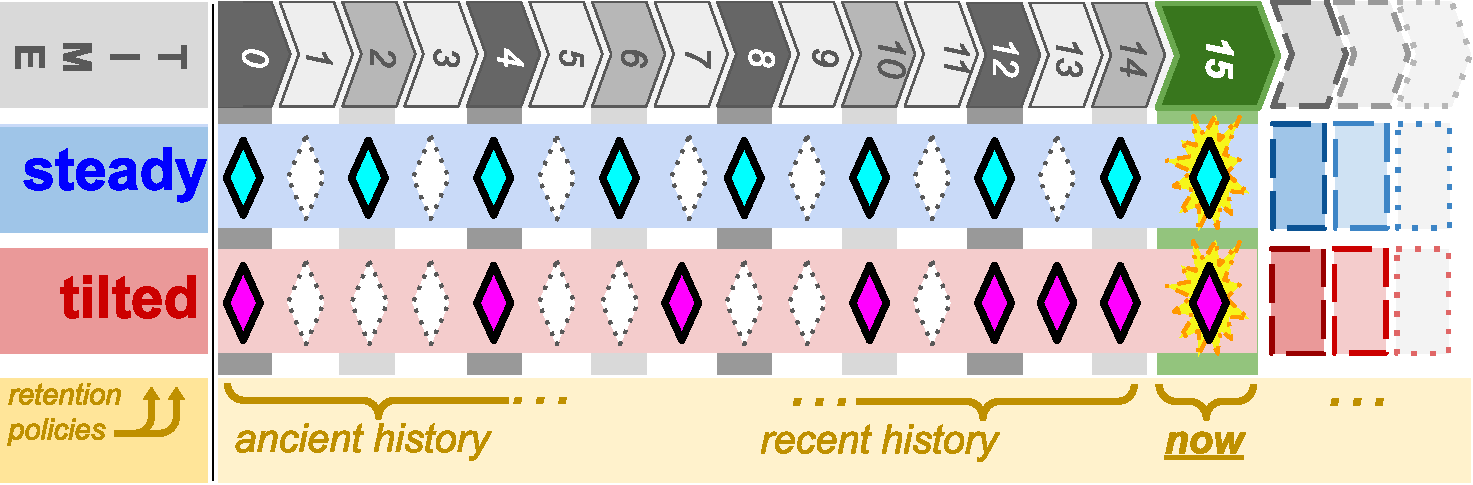
\includegraphics[width=\linewidth]{img/steady-vs-tilted-schematic}
  \caption{%
  \textbf{Steady versus tilted retention policy.}
  \textbf{\textit{Steady policy}} (top) retains differentia with time points spaced evenly across history.
  \textbf{\textit{Tilted policy}} (bottom) retains differentia more densely over recent history, giving gap size proportional to time ago.
  Retained differentia are shown as filled diamonds and discarded differentia are shown as empty.
  \textbf{\textit{Hybrid policy}} (not shown) allocates half of available space to hold tilted data and half to hold steady.
  }
  \label{fig:steady-vs-tilted-schematic}
\end{figure}
